\documentclass{article}
\usepackage[margin=1.2in]{geometry}
\usepackage{parskip}
\usepackage{amsthm}
\usepackage{amssymb}
\usepackage{amsmath}
\usepackage{cite}
\usepackage{graphicx}
\usepackage{epsfig}
\pagestyle{plain}
\topmargin -0.8in
\textheight 9.0in
\oddsidemargin -0.1in
\textwidth 6.8in

\title{\textbf{CS676: 3D Reconstruction from Several Images(Structure from Motion)\\} Report}
\author{\normalsize Anshu Avinash 10327122 \\ \normalsize Pranjal Singh 10327511\\ \normalsize Sunil Kumar 10327742\\
\emph{Indian Institute of Technology,Kanpur}\\ Advisor: Prof. Vinay P. Namboodiri}

\date{\today}
\begin{document}
\maketitle
\begin{abstract}
In this work we show how 3D reconstruction, basically structure from motion, from point correspondences of multiple images can be achieved. The original contributions with respect to related works in the field are mainly a direct global method for relative 3D reconstruction and a geometric method to select a correct set of reference points among all image points. Experimental results from real image sequences are presented, and algorithm has been discussed in detail.
\end{abstract}

\section{Introduction}
3D reconstruction from multiple images is the creation of three-dimensional models from a set of images. It is the reverse process of obtaining 2D images from 3D scenes.\\
Structure from motion (SfM) is a range imaging technique; it refers to the process of estimating three-dimensional structures from two-dimensional image sequences which may be coupled with local motion signals.\\
We humans perceive information about 3D structure in the environment by moving through it. When the observer moves and the objects around him move, information is obtained from images sensed over time.\\
We expect that our future will be full of robots, so these robots must have ability to perceive 3D structure like us. Hence, this work is motivated by this observation. The problem of SFM can be mathematically described as follows:\\
Given many points in correspondence across several images, $\{(u_{ij},v_{ij})\}$, simultaneously compute the 3D location $x_i$ and camera (or motion) parameters $(K,R_j,t_j)$\\
$\bar{u_{ij}}=f(K,R_j,t_j,x_i)$\\
$\bar{v_{ij}}=g(K,R_j,t_j,x_i)$

\section{Algorithm}
The basic framework and algorithm of this work can be understood by the following figure:\\\\
\includegraphics[width=130mm,height=80mm]{3.eps}\\\\
Now we will discuss each step in some detail.

\subsection{Feature Matching}
Feature matching is an integral part of SFM because we need to know the exact location of each point in every image sequence that we have so that we can project the same in 3D.\\
The geometrical theory of structure from motion assumes that one is able to solve the correspondence problem, which is to identify points in two or more views that are the projections of the same point in space.\\
One solution is to identify corresponding points interactively in each view. An important advantage is that surfaces can be defined simultaneously with correspondences. Feature matching works by detecting interest points in the images.\\
We have used \textbf{SIFT}(Scale Invariant Feature Transform) for feature extraction and k-NN for matching.\\
Optical flow is another alternative to get better matching. It is the process of matching selected points from one image to another, assuming both images are part of a sequence and relatively close to one another. Its advantageis that it is usually faster and can accommodate matching many more points, making the reconstruction denser. We have also experimented with Optical flow technique.

\subsection{Camera Calibration}
Camera intrinsic and extrinsic parameters can be determined for a particular camera and lens combination by photographing a controlled scene. We have assumed that our camera is calibrated, hence we know its intrinsic parameters such as focal length, optical center, aspect ration, etc.

\subsection{Fundamental Matrix-F}
It records motion between cameras and we have used RANSAC for calculation of $F$. The mathematical condition for determining $F$ is $x'Fx=0$.\\
It is used to calculate Essential Matrix which is described below.

\subsection{Essential Matrix-E}
$E=K^T \times F \times K$\\
It is $3 \times 3$ sized matrix which can be used to recover projection matrix for each camera. It imposes a constraint between a point in one image and a point in the other image with $x' \times E \times x=0$\\
where $x$ is a point in image one and $x'$ is the corresponding point in image two.

\subsection{Projection Matrix-P}
It is $3 \times 4$ sized matrix which contains rotation and translation parameters of the camera. It is derived by doing \emph{Singular Value Decomposition} of the \emph{Essential Matrix}.

\subsection{Triangulation}
Given projection matrices, 3D points can be computed from their measured image positions in two or more views. This is
triangulation. Ideally, 3D points should lie at the point of intersection of the back-projected rays. However,
because of measurement noise, back-projected rays will not generally intersect. Thus 3D points must be chosen in such a way as to minimize an appropriate error metric.\\
We have used \emph{Linear Method} for triangulation. Two key equations arising from the 2D point matching and $P$ matrices are:\\
$x=PX$ and $x'=P'X$\\
where $x$ and $x'$ are matching 2D points and $X$ is a real world 3D point.\\
If we rewrite the equations, we can formulate a system of linear equations that can be solved for the value of $X$, which is what we desire to find.

\subsection{Reconstruction from Many Views}
Now that we know how to recover the motion and scene geometry from two cameras, it would seem trivial to get the parameters of additional cameras and more scene points simply by applying the same process. This matter is in fact not so simple as we can only get a reconstruction that is up-to-scale, and each pair of pictures gives us a different scale.\\
There are a number of ways to correctly reconstruct the 3D scene data from multiple views. One way is of resection or camera pose estimation, also known as Perspective N-Point(PNP), where we try to solve for the position of a new camera using the scene points we have already found.\\
We have used $SolvePnPRansacfunction$ available in \emph{OpenCV}.

\subsection{Refinement of Reconstruction}
One of the most important parts of an SfM method is refining and optimizing the reconstructed scene, also known as the process of \emph{Bundle Adjustment}. This is an optimizing step where all the data we gathered is fitted to a monolithic model. Both the position of the 3D points and the positions of cameras are optimized, so re-projection errors are minimized (that is, approximated 3D points are projected on the image close to the position of originating 2D points).\\
We have used SSBA(Simple Sparse Bundle Adjustment) Library.

\subsection{Visualization}
We have used Point Cloud Library (PCL) for visualization of 3D points.

\section{Dataset Used}
We have used two datasets of CVlab of EPFL which are:
\begin{itemize}
\item Fountain P-11 Sequence \emph{http://cvlabwww.epfl.ch/\~strecha/multiview/denseMVS.html}\\
\includegraphics[width=120mm,height=60mm]{1.eps}
\item Herz-Jesu-P8 \emph{http://cvlabwww.epfl.ch/\~strecha/multiview/herzjesu\_dense.html}\\
\includegraphics[width=120mm,height=60mm]{2.eps}
\end{itemize}

\section{Result}
The following images shows our output on the two datasets of CVlab of EPFL:
\begin{itemize}
\item Fountain P-11 Sequence
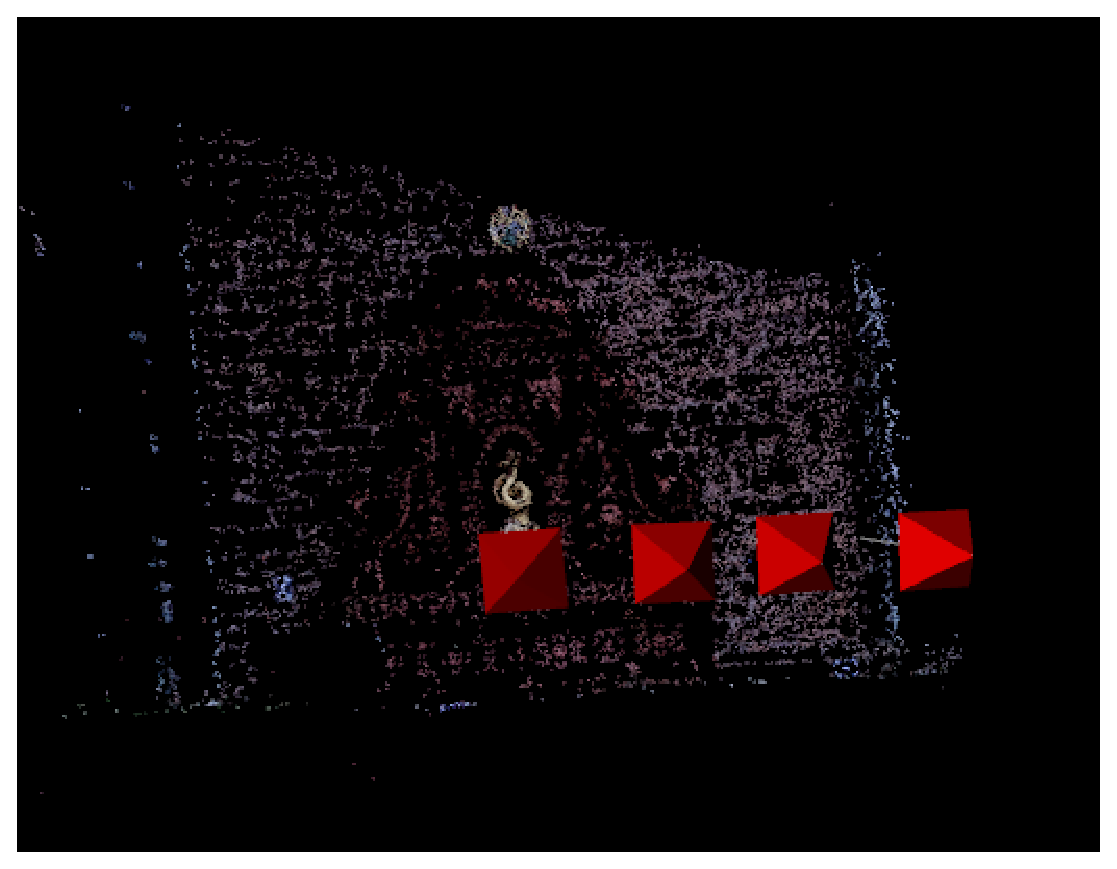
\includegraphics[width=80mm,height=50mm]{4.eps}
\item Herz-Jesu-P8

\includegraphics[width=80mm,height=50mm]{5.eps}
\end{itemize}

\section{Conclusions and Future Work}
In this paper we have presented a novel tool, which enables us to solve the structure from motion problem
without a priori correspondence information. The final algorithm is simple and easy to implement and fast.\\
The quality of results can be easily improved if we use more images from different views though it slows down the rate of computing. We can also improve if we have better feature correspondences in all images, implying that we can try with other feature extraction techniques.\\
The triangulation method that we have used is a linear method, we can experiment with other triangulation methods and then compare our results. There are also many state-of-the-art techniques available such as Bundler, VisualSFM,LibV. We can try to incorporate their techniques into our system.

\nocite{*}
\bibliography{report}{}
\bibliographystyle{plain}

\end{document}
